\section{Neural network implementation and models}
Building neural network for classifying pain maps was try and error process.
In this project the deep learning method is used to classify the pain maps and gender by determined outputs. The data is a set of 2D-images combined with gender and the outputs are pain intensity and duration. For classification purpose supervised convolutional neural network is used followed by fully-connected layers at the end. This architecture of the model is chosen to the interest of morphology and location of the pain. as there was no "golden recipe" for most optimized  The models are trained and tested on a single computer with GPU and ran on Python programming language with Keras library and Tensorboard tool for visualizing results. Specifications of hardware and software are described in detail in section {Sofware and hardware}.

\subsection{Software and hardware}
The neural network developed for this study, was programmed using Python v3.6.3. Python is an object-oriented and general-purpose programming and scripting language, that may be used for e.g. programming websites, mobile applications, but also for machine learning programming applications.
For development of deep learning application in python, different libraries are available, where some of the popular are the Theano and TensorFlow libraries.\citep{Swamynathan2017}, where the Tensorflow v1.3.0 library was used in this study. %TensorFlow is an open source library for development of machine learning applications, that has been released by Google \citep{Swamynathan2017}.  
An additionally library, Keras v2.0.8, was imported, which runs on top of either Tensorflow or Theano, and is a high-level neural networks application programming interface (API).   
Keras is a simplified version of the two libraries, which allows for fast and easier prototyping of neural network \citep{fcollet2015}. This was deemed suitable given that no previous experience with neural network were available during this study.  

Utilization of graphics processing unit (GPU) computation was also implemented using CUDA drivers and cnDNN communication libraries, which allowed for faster runtimes, then through the use of the central processing unit (CPU).
 
%Keras is a simplified version of the two libraries, which makes it easier to program in Python, but still allows for building complex models. TensorFlow is an open source library for development of machine learning applications, that has been released by Google \citep{Swamynathan2017}. 
%Using CPU or GPU on this platform the most mathematical operation  is computed in a computerized and simple way \citep{Swamynathan2017}. A small example of the concept of using TensorFlow could be seen in Appendix B. The plots for this model are generated using Tensorboard visualizing tool. It allows to watch a graph during the training, gives plot quantitative metrics and shows data like images that pass through it. Besides visualizing part of this tool it is also useful for debugging as it allows to observe the graph at a present time.\citep{Abadi2016a}

\noindent
The neural network was created on a laptop with 4x 'Intel® Core™ i7' CPU‘s and one GPU of type 'Geforce GTX 970M' with specifications listed in table \ref{tab:Specs}.

\begin{figure} [H]
\centering
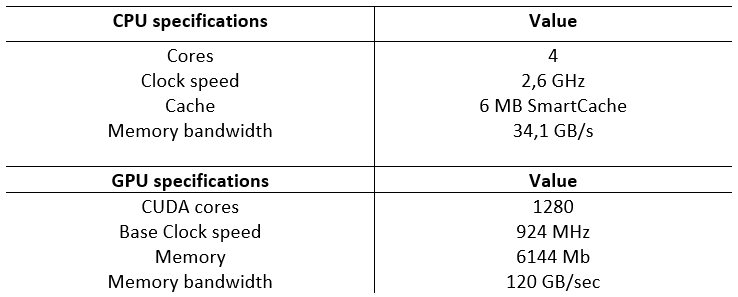
\includegraphics[width=1\textwidth]{figures/Specs}
\caption{Specifications of CPU‘s and GPU \citep{Intel,Nvidia}.}
\label{tab:Specs}
\end{figure}

\subsection{Data handling and design choices of the models}
This section presents the different models used, their architecture and implementation.
The models will be operating on a pixel level by learning features of the pain charts.
Each model will be using fully connected layer concept discussed in \autoref{sec:Layers}, and equal optimization methods. Convolutional layers will be used only on morphology and combined representations of data, while region representation containing labelled knee areas runs on fully connected layers.
Instead of including all pain maps from the dataset, validation and test set were specified separately. 10-fold cross validation technique were used calculate the average accuracy, specificity and sensitivity. Each model will be used twice to independently test the generalization performance of pain duration and intensity. Supervised learning is used for training in all the models. The generic input for all of the model is gender, along with the different image representation, which are presented in figure \ref{fig:Schema1}. These inputs are trained and then compared against their respective category label. 

\begin{figure} [H]
\centering
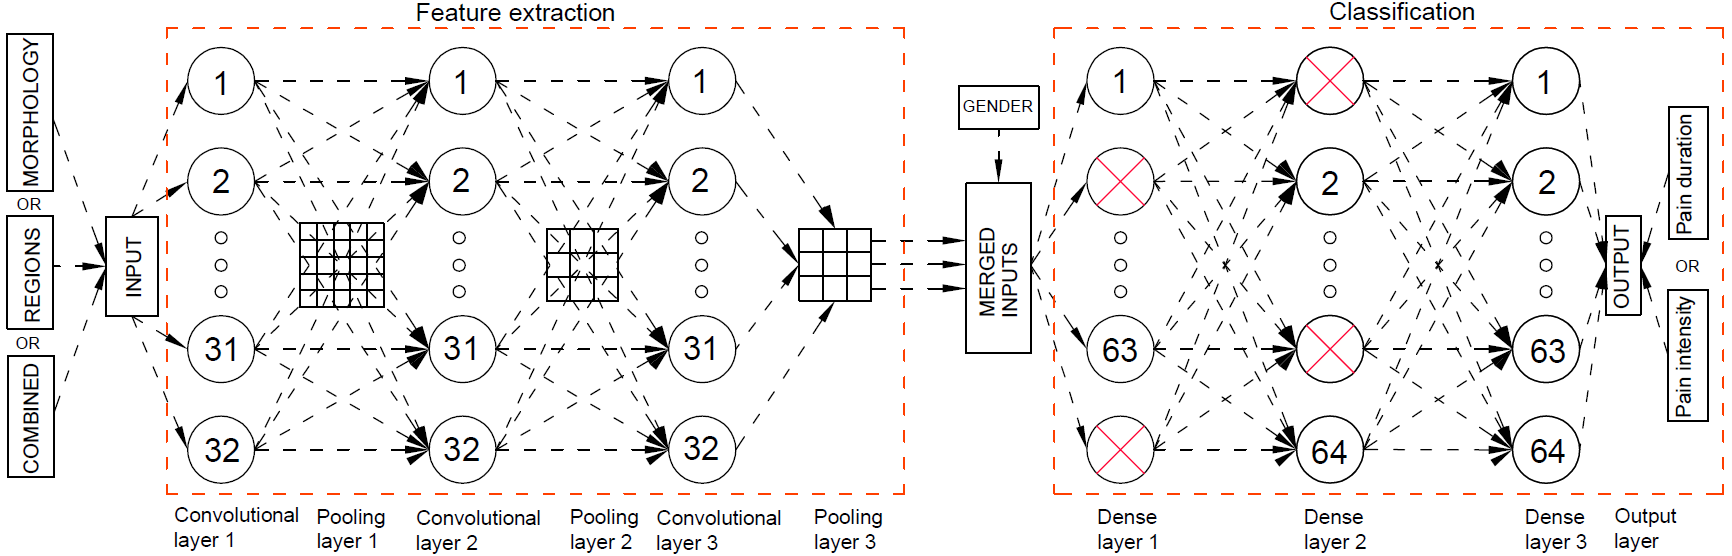
\includegraphics[width=1.0\textwidth]{figures/Schema1}
\caption{Architecture of the neural network model used for this study.}
\label{fig:Schema1} 
\end{figure}

From the higher point of view, the model can be architecturally split into two main parts. Feature extraction part, where convolutional and pooling layers alternates in order to extract the most important features out of the image. Second part is called classification, where computed feature maps will be assigned to particular class of the output layer. In order to obtain a higher generalization performance of deep learning classifier, methods like activation function, regulation and optimization will be used within the layers were implemented into the models.

\subsubsection{Morphology - representation model}
The pain map representation of morphology works as input of the model, where the input layer is a convolution layer. This layer is set-up to receive a input shape of the dimension of the pain map, that is defined during re-scaling of the pain maps in \ref{sec:Morph}. Gender works as secondary input in the second section of the model, along with the pain maps features extracted through the convolution layers. Before the pain maps features reach the fully connected layers it is flattened from a matrix to a single row in order to merge the features with gender. The merged data passes through fully connected layers and reaches the output layer where it is given a percentage value according to which class it fits the most. Morphology model architecture is shown in figure \ref{fig:Schema1}.

\subsection{Regions-representation model}
The architecture for this model only contains fully connected layer, since the data representation only contains 21 element vector that reflects the active pain regions and gender as described in \ref{sec:Regions}. It is evaluated that there would not be any gains in making the model more complex e.g. adding of convolution, based on the information available from vector, since the level of detail in relation to morphology is very simple. The architecture of the model is illustrated in \ref{fig:Simpleschema}.

\begin{figure} [H]
\centering
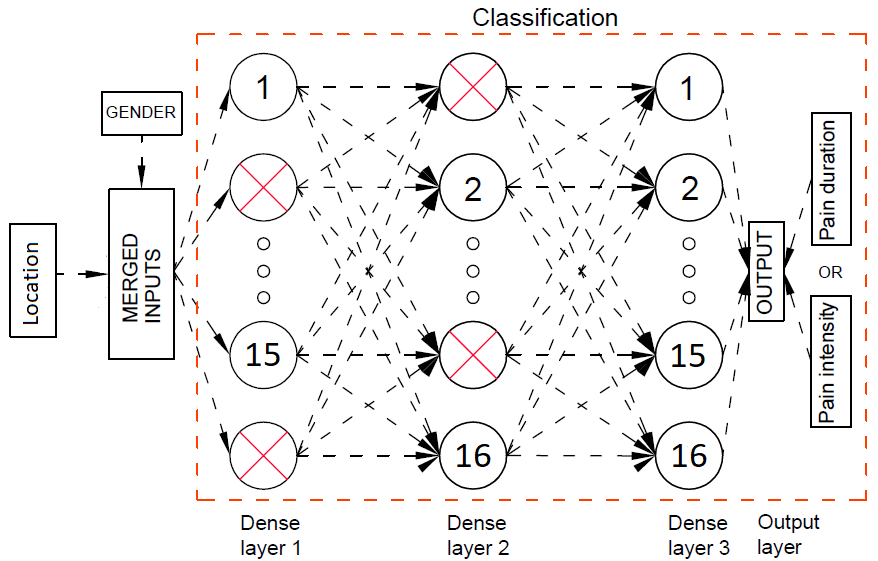
\includegraphics[width=0.6\textwidth]{figures/Simpleschema}
\caption{Architecture of the regions-representation model.}
\label{fig:Simpleschema} 
\end{figure}

\subsection{Combined representation model}
The architecture of this model is nearly identical to that of the morphology representation model.
The main difference can only be seen in the input layer for the pain map representation, where the input shape is altered to contain 20 layers per pain chart instead of one. This is the result of the one-hot encoding done to the images as described in \ref{sec:combined}. 

\subsection{Data handling in python}
The pre-processed data is loaded from a %\textip{.mat} 
.mat file into python.
Data within the file is pre-shuffled and split into a training and test sets, as described in \autoref{sec:pre-process}. The reason for shuffle the data is to improve generalisation through randomization.
In Python the training subset is further divided into a training and validation subsets. 
The training subset is used to find the optimal weights with the backpropagation algorithm \citep{Bengio2012}. In this project, training subset is considered to use up to 75\% of the data. The validation set makes up 15\% of the available data.
The test set will be used to evaluate the generalization of the model, and therefore will not contain data that has been used during the training. By keeping the test set separate it will act as new unseen data, for the model. It contains 10\% of the data.
For the morphology, and combined pain map representations, the images were reshaped from a row vector, back into a matrix to retain their 2D structure.
Furthermore the classification labels were one-hot encoded, so they were compatible to the number of outputs in the models. This is a result of the loss function \textit{categorical\_crossentropy} used for the models, that tries to reduce loss between the categories.    

\section{Optimization}
To try to reduce overfitting and improve generalization of the neural network different techniques are applied network models. Grid search method was used to find most optimal hyperparameters by cross-validating them 5 times and evaluating the mean values with SD. Activation function, dropout, optimizer, learning rate, type of initializer, number of neurons, batch size and number of epochs were tested using this method.  All used optimization techniques are presented in this section and table with used values is presented in FIGURE or RESULTS section (x,x)

\subsubsection{Activation function}
During this study different activation functions, such as ReLu, Softmax, Sigmoid were tested. Results were compared using grid-search and ReLu was picked as activation function for the models. Activation function was implemented in convolutional and fully-connected layers. Sigmoid activator was used for final output layer, because (NEED TO EXPLAIN).

\subsubsection{Dropout}
Dropout is implemented in the models due to the benefits described in section \ref{sec:dropout}. Dropout of three different values were tested on grid-search and 0.5 were picked as it scored the highest. This regulator is only used within the hidden fully-connected layers, where it is defined to randomly drop 50 \% of the nodes. Dropout is shown in figure \ref{fig:Simpleschema} and marked as red crosses. 

\subsubsection{Optimizer}
Adam, RMSprop, Adagrad and SGD, presented in section \ref{sec:optimizers}, were tested and compared. SGD scored the highest and was implemented while compiling the model.

\subsubsection{Learning rate}
In order to determine the most optimal \textit{learning\_rate} for the Adam  and SGD optimizers several different values were tested. Default value 0,001 performed higher than values of 0,01 and 0,0001. To fit the model this parameter was set to 0,001 meaning that the convergence of gradient descent is reached slower but with more accurate \textit{minima}. 

\subsubsection{Batch size and number of epochs}
Three different values of batch size and number of epochs were chosen based on computing power. Grid search on batch size were tested on 5, 10, 15 values, while number of epochs were 15, 25, 35. On every data representations these hyperparameters varied. Batch size and number of epochs were used during the fit process.

\subsubsection{Weight and biases initializing}
Weights and biases initialization was performed, since it affects the performance of the model.
A grid search of weight initializer using \textit{uniform}, \textit{lecun\_uniform}, \textit{normal}, \textit{glorot\_normal} and \textit{glorot\_uniform} were tested and results revealed that \textit{glorot\_normal} performed the best by 3,2 \% compared to the second best. Results can be seen in \ref{pictureFromCMD}. Weight initializer was used in convolutional and fully-connected layers.
Biases were initialized to zeros values
% See image - kernal_init.png 

\subsubsection{Number of neurons}
Number of neurons were chosen based on the best performance comparing 16, 32, and 64 neurons per hidden layer. 32 in convolutionals and 64 neurons in fully-connected layers scored the highest in terms of accuracy. These values were used in in the model within all data representations.

\subsection{Training and validation}
The training was performed using mini-batches of size 10 with SGD optimizer with default learning rate, explained in section \ref{sec:optimizers}. Data was split into train(75\%), validation (15\%), and test (10\%) sets, and the models were regularized using dropout (50\%). Number of neurons in hidden layers were decided to be used as 32 for convolutional and 64 for fully-connected layers. All networks were using ReLu activation function, except output layers, which were using Sigmoid activator instead, described in Section %{activation function}.
The model weight parameters were initialized at random values using \textit{glorot\_normal}, biases parameters were initialized to zero values.

\subsubsection{Stratified m-folds cross-validation}
As a result of binary output, 10-fold cross-validation method were used for training the data and evaluating the performance of the models. Folds were separated 10 times randomly in relation to the distribution of the classes. Stratified m-folding prevents the fold to contain the data of one class. Accuracy, sensitivity and specificity were calculated after each fold and the mean values of these parameters were generated at the end of the training. Results are given in section %{the results}.

\subsubsection{Error and accuracy graphs)}
During each training and validating epoch, the error and accuracy is calculated and presented as graph at the end. According the error graph, the overfitting or underfitting could be determined. Model could be optimized based on these results with technique described in section \ref{sec:optimizers}.

\subsection{Testing}
The testing or prediction refers the generalization performance from the given classification question and is the main job for the neural network.
Separated 10\% dataset were used for testing how accurate the training model can perform using unknown data. By feeding new data into the network, testing process begins. At each time-step classifier predicts the probability for every possible class, and selects with the highest probability as it prediction, giving it as a percentage result. Predictions were presented as a confusion matrix in section {results} providing true positive and negative together with false positive and negative results.
